\subsubsection{Dimensiones del área de trabajo}

El sistema robótico presenta una configuración cartesiana de dos ejes (XY), con dimensiones de 3~m de ancho por 2~m de alto, diseñado para operar sobre cultivos hidropónicos verticales dispuestos en tubos montados sobre una pared.

\subsubsection{Especificaciones cinemáticas}

Las especificaciones de velocidad, aceleración y resolución de los actuadores se detallan en la Tabla \ref{tab:esp_cinematicas}.

\begin{table}[htbp]
\centering
\begin{tabular}{|l|c|c|}
\hline
\textbf{Parámetro} & \textbf{Eje Horizontal} & \textbf{Eje Vertical} \\ \hline
Velocidad máxima [\(\frac{mm}{s}\)] & 250 & 75 \\ \hline
Velocidad mínima [\(\frac{mm}{s}\)] & 12.5 & 2.5 \\ \hline
Aceleración [\(\frac{mm}{s^2}\)] & 187.5 & 45 \\ \hline
Avance por revolución [\(\frac{mm}{rev}\)] & 40 & 8 \\ \hline
Resolución [\(\frac{pasos}{mm}\)] & 40 & 200 \\ \hline
Micropasos & 8 & 8 \\ \hline
\multicolumn{3}{c}{} \\
\end{tabular}
\caption{Especificaciones cinemáticas de los ejes de movimiento}
\label{tab:esp_cinematicas}
\end{table}

La diferencia en resolución entre ambos ejes responde a los requisitos operativos: el eje horizontal requiere mayor velocidad de desplazamiento con precisión moderada, mientras que el eje vertical necesita mayor precisión de posicionamiento con velocidades menores debido a las operaciones de elevación de carga.

\subsubsection{Cargas del sistema}

Las cargas consideradas en el diseño se distribuyen según su función operativa:\\

Cargas del eje horizontal.\\
\noindent
El motor del eje horizontal debe mover aproximadamente 12~kg, correspondiente a la suma del peso de las varillas verticales, la varilla roscada, los soportes estructurales y el brazo robótico. La carga es soportada principalmente por el perfil superior.

Cargas del eje vertical.\\
\noindent
El motor del eje vertical debe mover la carga correspondiente al peso del brazo robótico y la lechuga. Además, debe vencer la fricción que se genera entre la tuerca y la varilla roscada.

\subsubsection{Componentes estructurales}

El robot cuenta con tres soportes estructurales principales fabricados mediante impresión 3D:

\begin{itemize}[label=$\bullet$]
    \item \underline{Soporte inferior:} Fijación de las varillas verticales y montaje del motor del eje Z
    \item \underline{Soporte medio:} Sostiene el brazo robótico y la cámara, desplazándose verticalmente mediante la varilla roscada
    \item \underline{Soporte superior:} Acoplamiento cinemático de los dos movimientos perpendiculares (horizontal y vertical), actuando como elemento de unión entre ambos subsistemas
\end{itemize}

El motor del movimiento horizontal estará sostenido por un soporte como el mostrado en la fig. \ref{fig:soporte_motor_pap}
\begin{table}[H]
\centering
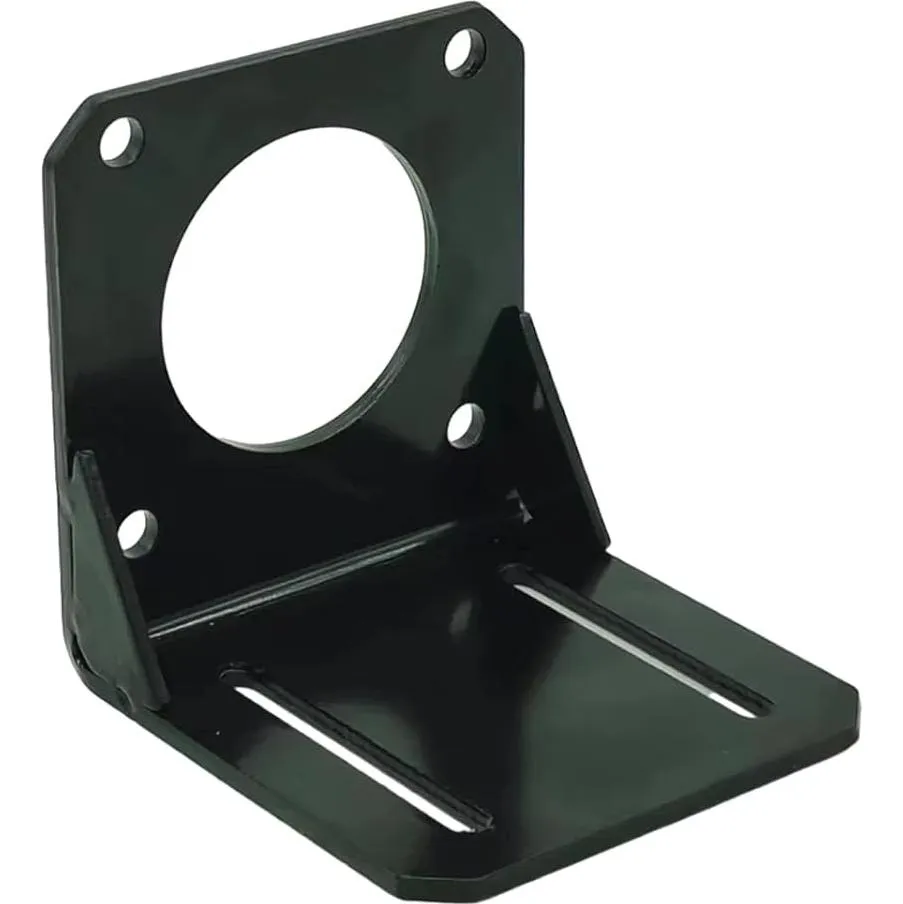
\includegraphics[width=0.25\textwidth]{img/soporte_motor_pap.png}
\caption{\textit{Referencia de oporte para motor pap.}}
\label{fig:soporte_motor_pap}
\end{table}
El perfil superior se une a un caño estructural en cada extremo utilizando soportes tipo L. Mientras que el perfil lateral que brinda rigidez, se atornilla también a un tramo de caño estructural en cada extremo. Las orientaciones de los caños estructurales de soporte se puede observar en la fig. \ref{fig:ClaudioReal_simplificado}